\chapter{Alignments with Pair HMMs}

In this chapter we will describe scoring schemes for pair alignment using PHMMs.
We can divide states of PHMM into three types.  Ones that generates symbol in
both sequences, states that generates symbol in only one sequence and silent
states. If PHMM generates  symbols in both sequences we consider those symbols
to be homologous. We will consider symbols that were not generated by such state
as indels.

If we have sequences $X$ and $Y$, probability $\prob{X,Y\mid H}$ is the
probability, that $X$ and $Y$ are aligned according model $H$. Since from state
path $\pi$ we can reconstruct unique alignment, we will denote $\pi$ also as an
alignment. $\prob{\pi\mid X,Y,H}$ is the probability, that $\pi$ is alignment of
$X$ and $Y$ under the condition, that $X$ and $Y$ were generated by model
$H$. We can use $\prob{\pi\mid X,Y,H}$ as a score of an alignment $\pi$. Later
in this chapter we show how to derive different scoring functions.


\section{Simple Pair HMM Model}

We show classical PHMM for sequence alignment. It is equivalent to scoring
scheme of Needleman-Wunch algorithm with affine gap model. It consists of three
states: one that generates aligned pairs, and two states for generating
indels (one for each sequence). Model is shown in figure \ref{PHMM:FIG:SIMPLEPHMM}. 

\begin{figure}[Simple pair HMM model for alignment.]
\begin{center}
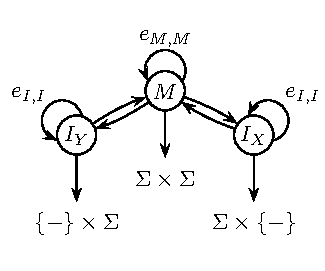
\includegraphics{../figures/pairHMM.pdf}
\end{center}
\caption{Pair hidden Markov model for pair alignment. It has two transitions
parameters $e_{M,M}$ and $e_{I,I}$, since we set $e_{I,M} = 1 - e_{I,I}$ and
$e_{M,I}=\frac12-\frac12e_{M,M}$. Match state $M$ generates aligned pair of symbols
and states $I_X$ and $I_Y$ generates symbols only in $X$ or $Y$ respectively.
Initial distribution is even.
}\label{PHMM:FIG:SIMPLEPHMM}
\end{figure}

As mentioned before, score of the alignment is the probability of state path
that correspond to such alignment. Therefore we can find the alignment with 
highest score by two dimensional version of Viterbi algorithm. 

\section{More Complex models}

In this section we will review several PHMMs and GPHMMs that were used to
sequence alignment or other purpose, for example gene finding. We will review
the application domain of the model, its topology, decoding function,
parameter estimation and optimisation heuristics.

\subsection{SLAM}

SLAM is comparative-based gene finder \cite{SLAM2003} based on generalized pair hidden
Markov model \cite{Alexanderson2004}. It predicts gene structures for pair of
related eukaryotic organisms. SLAM's decoding method is Viterbi algorithm. 


Emission of pairs of codons were assigned from codon-based PAM matrix.

To reduce running time of the algorithm, they restrict computation of alignment
in following way. At first they  align input sequences using AVID alignment
tool. After that they relaxed alignment in a way, that every pair of aligned
bases were extended to intervals of size $3$ bases of bases surrounding each
matching base.


\subsection{GeneWise}
\subsection{FEAST}
\subsection{Doublescan}
\subsection{Twine}
\subsection{Pairagon}

\section{More Complex Gap Models}
Gapmodel defined by PHMM is in fact affine gapmodel.
Gap length have geometric distribution: the probability that gap have length $d$
is $e_{M,I}e_{I,I}^{d-1}(1-e_{I,I})$ (if we sum out all emissions). However,
using
%co chcem povedat: niekedy je lepsie pouzit iny gapmodel -- jeden pre kratke
%gapy, jeden pre slhe gapy. Preto sa niekedy 

\section{Multiple Rates of Evolution}

We can define alternative function 
